\documentclass{article}

\usepackage{Sweave}
\begin{document}
\Sconcordance{concordance:WC86.tex:WC86.Rnw:%
1 2 1 1 0 20 1 1 2 1 0 1 1 3 0 2 2 4 0 2 2 1 0 2 1 3 0 2 2 4 0 2 2 4 0 %
1 2 1 1 1 2 6 0 2 1 6 0 2 2 27 0 1 2 10 1 1 4 1 2 5 1 1 2 8 0 2 2 6 0 2 %
1 6 0 2 2 4 0 1 2 1 1 1 2 48 0 1 2 10 1 1 2 4 0 2 2 6 0 2 1 6 0 2 2 1 0 %
1 1 5 0 2 1 6 0 1 2 2 1 2 3 6 1 1 3 1 2 9 1 1 4 3 0 1 3 2 0 1 3 5 0 1 2 %
13 1 1 4 3 0 1 3 2 0 1 3 5 0 1 2 26 1}


\title{Analysis of wallaby and kangaroo line transect data}
\author{David L. Borchers and Martin J. Cox}
\maketitle
\section{Summary}
\begin{enumerate}
  \item Data were collected by an observer walking line transects with a 400 m line spacing.
  \item Line transects were orientated east-west and north-south through the survey area.
  \item Two species were present in the survey area: wallaby and kangaroo.
  \item During the north-south transects the observer left the transect to confirm group size.
  \item Data were split by species and transect direction.
  \item So far data have be analysed for wallaby and kangaroo for the east-west transects using the 'h1' hazard function form and uniform and half-normal perpendicular density gradients ($\pi_x$,Tables \ref{tab:one} \& \ref{tab:two}).  The normal form for $\pi_x$ is a poor fit, resulting in either problems inverting the hessian (wallaby data set) or massive variance for the parameter estimates (kangaroo data set). 
  \item I have had no luck fitting the 'h2' hazard function, initial values seem to be the problem
\end{enumerate}

\section{Overview}
The wallaby and kangaroo sighting line transect data were provided by Colin Southwell in a Microsoft access database.  Here, we use data from Wallaby creek although other data sets are available. The Access database files were converted to xlsx files.  The two species analysed are the little wallaby (denoted as \texttt{RNW} in the files) and 'big' kangaroos (denoted as \texttt{EGK} in the files).  The wallabys are small and like dense habitat, whereas the kangaroos are comfortable in the open.  

\subsection{User defined variables}
\begin{Schunk}
\begin{Sinput}
> w=200 #m (half inter-transect spacing)
> ystart=400 #m  
\end{Sinput}
\end{Schunk}
We start by loading the \texttt{R} workspace with the model fit objects because I can't yet work out how to make Sweave cache:
\begin{Schunk}
\begin{Sinput}
> load('~/Dropbox/packages/2D distance sampling with time/data/landSurveys/workspace.RData')
\end{Sinput}
\end{Schunk}
Next we read in sightings and transect data.  To do so, we will need the \texttt{xlsx} package.
\begin{Schunk}
\begin{Sinput}
>   library(xlsx)
> transects=read.xlsx('~/Dropbox/packages/2D distance sampling with time/data/landSurveys/WC86TN.xlsx',sheetIndex=1)
> sightings=read.xlsx('~/Dropbox/packages/2D distance sampling with time/data/landSurveys/WC86IS.xlsx',sheetIndex=1)  
\end{Sinput}
\end{Schunk}
We make use of the \texttt{psych:scatterplot} function to display the sightings data.
\begin{Schunk}
\begin{Sinput}
> require(psych)
\end{Sinput}
\end{Schunk}
Source the package \texttt{R} code:
\begin{Schunk}
\begin{Sinput}
> source("~/dropbox/packages/2D distance sampling with time/R/2DLTfunctions.r")
\end{Sinput}
\end{Schunk}

The line transects were 400 m. Data were collected by observers on foot in the pre-GPS era, so no grid coordinates are available for the transects.  \textbf{I have a note from my discussions with Colin that the observer left the N-S and S-N direction transects, so we'll concentrate our analyses on the E-W and W-E transects.}  Remove the N-S and S-N transects.
\begin{Schunk}
\begin{Sinput}
> nrow(transects)
\end{Sinput}
\begin{Soutput}
[1] 78
\end{Soutput}
\begin{Sinput}
> transects=subset(transects,TDRN %in% c('EW','WE'))  
> nrow(transects)
\end{Sinput}
\begin{Soutput}
[1] 47
\end{Soutput}
\end{Schunk}
Examine transect data:
\begin{Schunk}
\begin{Sinput}
> summary(transects)
\end{Sinput}
\begin{Soutput}
      SIDT        TIDT            TNNU            TBRG       TDRN   
 Min.   :4   Min.   :12.00   Min.   : 7.00   Min.   : 90.0   EW:20  
 1st Qu.:4   1st Qu.:17.00   1st Qu.:26.50   1st Qu.: 90.0   NS: 0  
 Median :4   Median :21.00   Median :43.00   Median : 90.0   SN: 0  
 Mean   :4   Mean   :20.47   Mean   :42.21   Mean   :166.6   WE:27  
 3rd Qu.:4   3rd Qu.:24.50   3rd Qu.:58.50   3rd Qu.:270.0          
 Max.   :4   Max.   :28.00   Max.   :77.00   Max.   :270.0          
      TLGT             DATE                 TDUR       OBID         REPL      
 Min.   :0.5000   Min.   :1986-08-23   Min.   :17.00   CS:47   Min.   :3.000  
 1st Qu.:0.8250   1st Qu.:1986-08-28   1st Qu.:26.50           1st Qu.:3.000  
 Median :1.0000   Median :1986-08-30   Median :34.00           Median :4.000  
 Mean   :0.9649   Mean   :1986-08-28   Mean   :33.15           Mean   :3.574  
 3rd Qu.:1.1000   3rd Qu.:1986-08-31   3rd Qu.:39.00           3rd Qu.:4.000  
 Max.   :1.2000   Max.   :1986-09-02   Max.   :60.00           Max.   :4.000  
      TDAY      
 Min.   :1.000  
 1st Qu.:2.000  
 Median :2.000  
 Mean   :2.043  
 3rd Qu.:3.000  
 Max.   :3.000  
\end{Soutput}
\end{Schunk}
\begin{description}
  \item[SIDT] site ID.
  \item[TNNU] transect number
  \item[TBRG] transect bearing, deg (0 = north; 90 = east)
  \item[TDRN] transect direction, grid (e.g. east to west = EW)
  \item[TLGT] transect length, km
  \item[TDUR]  
\end{description}
We need the transects to be observed at a constant speed so checking transect speed:
\begin{figure}
\begin{center}
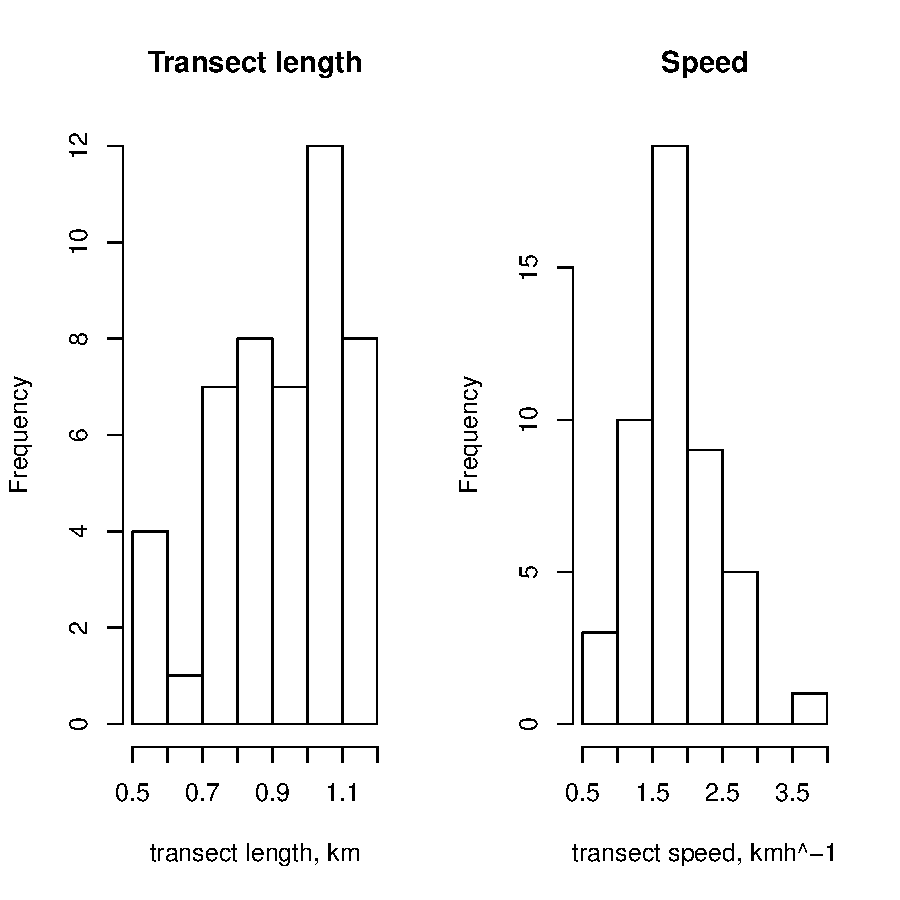
\includegraphics{WC86-fig1}
\end{center}
\caption{Transect lengths and survey speeds.}
\label{fig:one}
\end{figure}

and the direction of transects:
\begin{Schunk}
\begin{Sinput}
> table(transects$TBRG)
\end{Sinput}
\begin{Soutput}
 90 270 
 27  20 
\end{Soutput}
\end{Schunk}
We will now subset the observation data to include only EW and WE transects:
\begin{Schunk}
\begin{Sinput}
> nrow(sightings)  
\end{Sinput}
\begin{Soutput}
[1] 1124
\end{Soutput}
\begin{Sinput}
> sub.sight=subset(sightings,sightings$TNNU %in% unique(transects$TNNU))
> nrow(sub.sight)
\end{Sinput}
\begin{Soutput}
[1] 629
\end{Soutput}
\end{Schunk}
merge the sightings and transect data:
\begin{Schunk}
\begin{Sinput}
> sub.sight=merge(sub.sight,transects,'TNNU')
\end{Sinput}
\end{Schunk}
\subsection{Sightings data}
  
\begin{Schunk}
\begin{Sinput}
> summary(sub.sight)
\end{Sinput}
\begin{Soutput}
      TNNU           SIDT.x       STNU             HOUR        SPEC    
 Min.   : 7.00   Min.   :4   Min.   : 1.000   Min.   : 6.00   EGK:402  
 1st Qu.:29.00   1st Qu.:4   1st Qu.: 2.000   1st Qu.: 8.00   RNW:227  
 Median :44.00   Median :4   Median : 4.000   Median :12.00            
 Mean   :42.63   Mean   :4   Mean   : 4.095   Mean   :11.94            
 3rd Qu.:57.00   3rd Qu.:4   3rd Qu.: 6.000   3rd Qu.:16.00            
 Max.   :77.00   Max.   :4   Max.   :13.000   Max.   :17.00            
      ANGL            RADL            PERP             GPSZ       
 Min.   :  0.0   Min.   :  8.0   Min.   :  0.00   Min.   : 1.000  
 1st Qu.: 21.0   1st Qu.: 55.0   1st Qu.: 20.00   1st Qu.: 2.000  
 Median : 44.0   Median : 88.0   Median : 53.00   Median : 3.000  
 Mean   : 47.1   Mean   :101.7   Mean   : 64.69   Mean   : 5.124  
 3rd Qu.: 68.0   3rd Qu.:140.0   3rd Qu.: 89.00   3rd Qu.: 6.000  
 Max.   :168.0   Max.   :330.0   Max.   :249.00   Max.   :23.000  
      MVST              SBMV             FSAG            TWAW       
 Min.   :0.00000   Min.   :0.0000   Min.   :0.000   Min.   :0.0000  
 1st Qu.:0.00000   1st Qu.:0.0000   1st Qu.:0.000   1st Qu.:0.0000  
 Median :0.00000   Median :0.0000   Median :0.000   Median :0.0000  
 Mean   :0.08903   Mean   :0.4817   Mean   :0.787   Mean   :0.6216  
 3rd Qu.:0.00000   3rd Qu.:1.0000   3rd Qu.:1.000   3rd Qu.:0.0000  
 Max.   :9.00000   Max.   :9.0000   Max.   :9.000   Max.   :9.0000  
   HABT              GPRP            SIDT.y       TIDT            TBRG      
 Mode:logical   Min.   : 15.00   Min.   :4   Min.   :12.00   Min.   : 90.0  
 NA's:629       1st Qu.: 25.00   1st Qu.:4   1st Qu.:17.00   1st Qu.: 90.0  
                Median : 55.00   Median :4   Median :19.00   Median : 90.0  
                Mean   : 66.16   Mean   :4   Mean   :19.67   Mean   :176.7  
                3rd Qu.: 95.00   3rd Qu.:4   3rd Qu.:22.00   3rd Qu.:270.0  
                Max.   :255.00   Max.   :4   Max.   :28.00   Max.   :270.0  
 TDRN          TLGT            DATE                 TDUR       OBID    
 EW:303   Min.   :0.500   Min.   :1986-08-23   Min.   :17.00   CS:629  
 NS:  0   1st Qu.:0.900   1st Qu.:1986-08-28   1st Qu.:31.00           
 SN:  0   Median :1.100   Median :1986-08-30   Median :35.00           
 WE:326   Mean   :1.012   Mean   :1986-08-28   Mean   :37.46           
          3rd Qu.:1.100   3rd Qu.:1986-08-31   3rd Qu.:44.00           
          Max.   :1.200   Max.   :1986-09-02   Max.   :60.00           
      REPL            TDAY      
 Min.   :3.000   Min.   :1.000  
 1st Qu.:3.000   1st Qu.:1.000  
 Median :4.000   Median :2.000  
 Mean   :3.518   Mean   :2.052  
 3rd Qu.:4.000   3rd Qu.:3.000  
 Max.   :4.000   Max.   :3.000  
\end{Soutput}
\end{Schunk}
\begin{description}
  \item[ANGL] Sighting angle 0 = along transect; 90 - abeam
  \item[RADL] Range finder distance
  \item[PEPR] Perpendicular distance calculated from ANGL and RADL
  \item[GPSZ] Group size.
  \item[MVST] Movement: 0 = still; 1 = movement after detected.
  \item[SBMV] Subsequent movement, after detection
  \item[TWAW] 0 = away, 1 = towards \textbf{this is wrong}
\end{description}

Add a y-coordinate to each sighting:
\begin{Schunk}
\begin{Sinput}
> sub.sight$Y=sqrt(sub.sight$RADL**2-sub.sight$PERP**2)
\end{Sinput}
\end{Schunk}
Subset the sightings data based on truncation distance, $w$, and maximum y-coordinate range \texttt{ystart}:
\begin{Schunk}
\begin{Sinput}
> nrow(sub.sight)
\end{Sinput}
\begin{Soutput}
[1] 629
\end{Soutput}
\begin{Sinput}
> sub.sight=subset(sub.sight, PERP < w & Y <ystart)
> nrow(sub.sight)  
\end{Sinput}
\begin{Soutput}
[1] 612
\end{Soutput}
\end{Schunk}
Now we split the data by species:
\begin{Schunk}
\begin{Sinput}
> RNWdat=subset(sub.sight,SPEC=='RNW')
> nrow(RNWdat)
\end{Sinput}
\begin{Soutput}
[1] 223
\end{Soutput}
\begin{Sinput}
> EGKdat=subset(sub.sight,SPEC=='EGK')
> nrow(EGKdat)  
\end{Sinput}
\begin{Soutput}
[1] 389
\end{Soutput}
\end{Schunk}
Display the sightings
\begin{figure}
\begin{center}
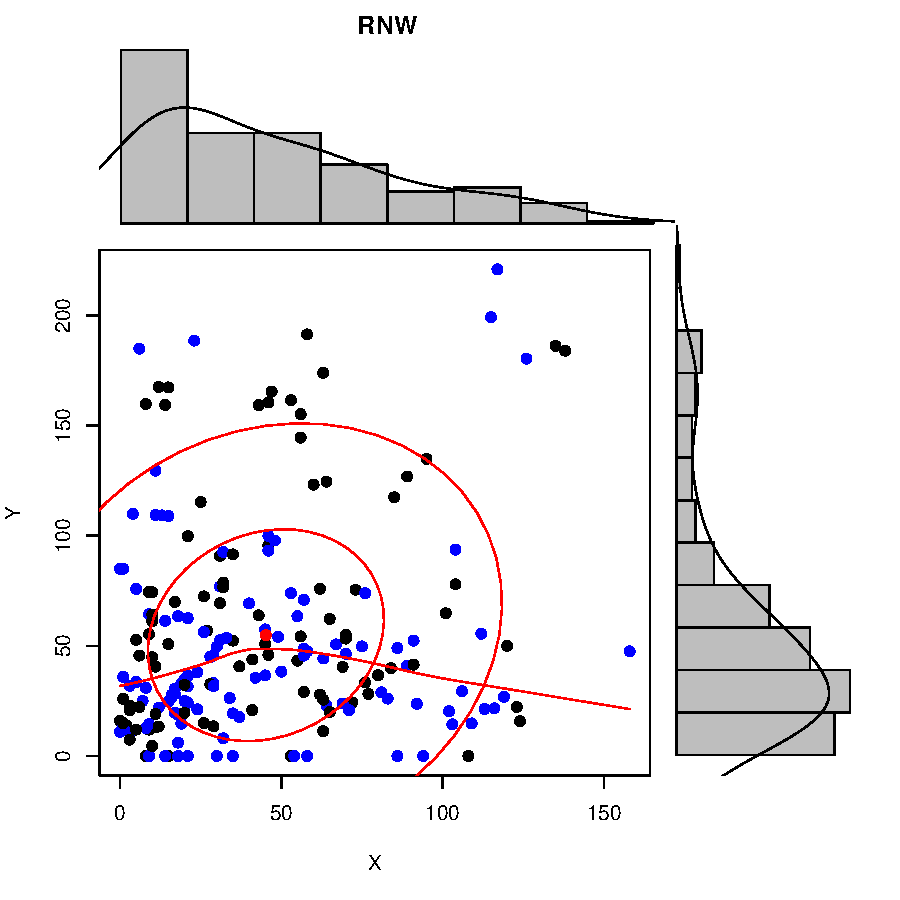
\includegraphics{WC86-fig2}
\end{center}
\caption{Observations for wallabys (RNW).}
\label{fig:two}
\end{figure}

\begin{figure}
\begin{center}
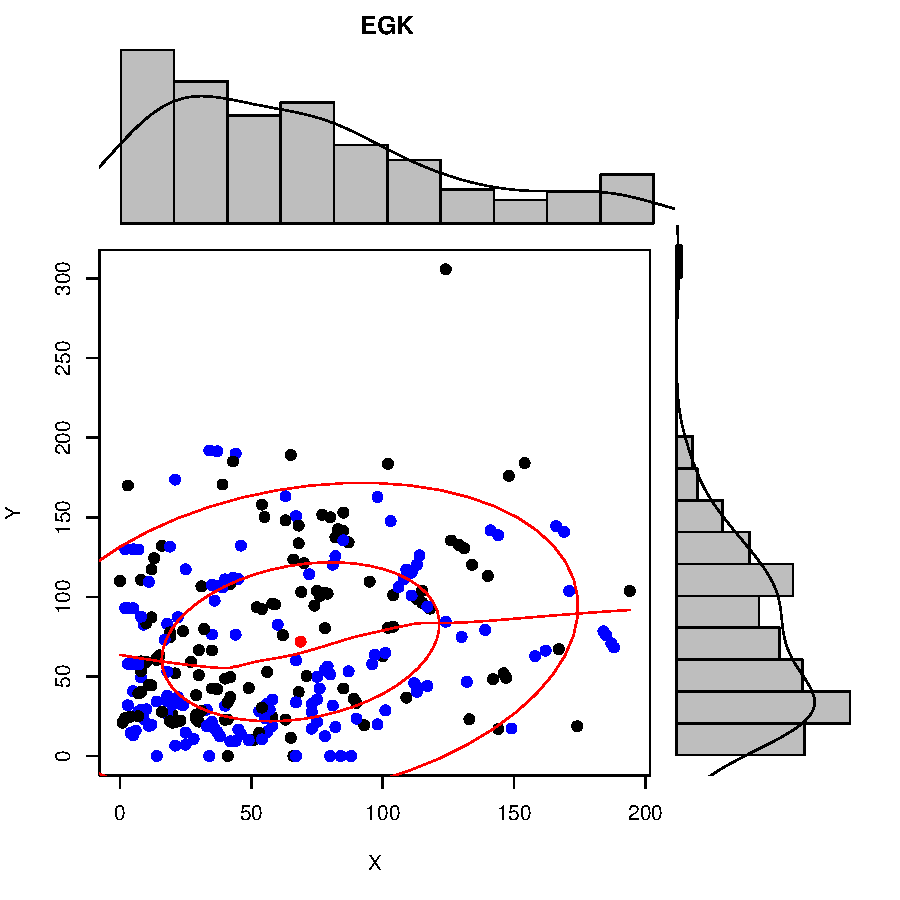
\includegraphics{WC86-fig3}
\end{center}
\caption{Observations for kangaroos (EGK).}
\label{fig:three}
\end{figure}



\section{Analysis}
In the analysis section we will attempt to fit three models to each species, each model will have a different perpendicular density distribution: (i) uniform; (ii) half-normal and (iii) normal.  We will use the 'h2' hazard rate form \textbf{I have had no luck fitting the 'h1' hazard rate function, initial values seem to be the problem}.
\subsection{Analysis of the EW and WE wallaby (RNW) sightings}
\begin{Schunk}
\begin{Sinput}
> #fit uniform perpendicular density function:
> modRNWunif=fityx(y=RNWdat$Y,x=RNWdat$PERP,b=log(c(1,1)),hr=h1,ystart=ystart,
+                  pi.x=pi.const,logphi=NULL,w=w,hessian=TRUE)
> #fit half-normal perpendicular density function:
> modRNWhn=fityx(y=RNWdat$Y,x=RNWdat$PERP,b=log(c(1,1)),hr=h1,ystart=ystart,
+                  pi.x=pi.hnorm,logphi=150,w=w,hessian=TRUE)
> #normal perpendicular density function:
> modRNWn=fityx(y=RNWdat$Y,x=RNWdat$PERP,b=log(c(1,1)),hr=h1,ystart=ystart,
+                  pi.x=pi.norm,logphi=c(0.1,10),w=w,hessian=TRUE)
\end{Sinput}
\end{Schunk}
\begin{table}[h!]
\caption{Wallaby (RNW) data set parameter estimates for the \texttt{h1} form of the hazard function and uniform and half-normal perpendicular density distribution.}\label{tab:one}
\begin{tabular} {c | c | c | c}
Density  & Hazard rate \texttt{h1}& $\pi_x$ & dAIC \\
distribution & parameters (CV) $\hat{b}$ & parameters (CV) $\hat{\phi}$ &  \\
\hline
Uniform & 5.02 ( 0.05 ); 0.92 ( 0.02 ) & - & 4.1\\
  
Half-normal & 4.75 ( 0.06 ); 0.89 ( 0.03 ) & 163.19 ( 0.23 )
& 0\\
\end{tabular}
\end{table}
\clearpage
\subsection{Analysis of the EW and WE wallaby (EGK) sightings}
\begin{Schunk}
\begin{Sinput}
> #fit uniform perpendicular density function:
> modEGKunif=fityx(y=EGKdat$Y,x=EGKdat$PERP,b=log(c(1,1)),hr=h1,ystart=ystart,
+                  pi.x=pi.const,logphi=NULL,w=w,hessian=TRUE)
> #fit half-normal perpendicular density function:
> modEGKhn=fityx(y=EGKdat$Y,x=EGKdat$PERP,b=log(c(1,1)),hr=h1,ystart=ystart,
+                  pi.x=pi.hnorm,logphi=150,w=w,hessian=TRUE)
> #normal perpendicular density function:
> modEGKn=fityx(y=EGKdat$Y,x=EGKdat$PERP,b=log(c(1,1)),hr=h1,ystart=ystart,
+                  pi.x=pi.norm,logphi=c(0.1,10),w=w,hessian=TRUE)
\end{Sinput}
\end{Schunk}
\begin{table}[h!]
\caption{Kangaroo (EGK) data set parameter estimates for the \texttt{h1} form of the hazard function and uniform and half-normal perpendicular density distribution.}\label{tab:two}
\begin{tabular} {c | c | c | c}
Density  & Hazard rate \texttt{h1}& $\pi_x$ & dAIC \\
distribution & parameters (CV) $\hat{b}$ & parameters (CV) $\hat{\phi}$ &  \\
\hline
Uniform & 4.68 ( 0.05 ); 0.83 ( 0.03 ) & - & 0\\
  
Half-normal & -51.08 ( NA ); 0.24 ( NA ) & 427.34 ( NA )
& 242\\
Normal & 4.68 ( NA ); 0.83 ( NA ) & 2.58 ( NA ); 12.51 ( NA )
& 2\\
\end{tabular}
\end{table}
\clearpage

\section{Next steps}
\begin{enumerate}
  \item Find out why $\pi_x$ normal distribution is failing.  
  \item Find out why hazard function form \texttt{h2} isn't working.
  \item Truncate the EGK data set at y=200 (see Fig. \ref{fig:three}).
  \item Look at speeds for North-South transects. Perhaps these are more consistent than East-West transects.
\end{enumerate}


\end{document}

